\section{Средства поддержки для разработки программного обеспечения (ПО) на смартфоне}
\subsection{Среда разработки приложений – операционная система Андроид}
Android (Андроид) — операционная система для смартфонов, интернет-планшетов, электронных книг, цифровых проигрывателей, наручных часов, игровых приставок, нетбуков, смартбуков, очков Google, телевизоров и других устройств. В будущем планируется поддержка автомобилей и бытовых роботов. Основана на ядре Linux и собственной реализации виртуальной машины Java от Google. В 86\% смартфонов, проданных во втором квартале 2014 года, была установлена операционная система Android. При этом за 2014 год было продано более 1 миллиарда Android-устройств \cite{android}.

\textbf{Преимущества операционной системы Android:}

\begin{itemize}
	\item Операционная система с открытым исходным кодом обладает большими преимуществами в возможностях настройках, и имеет возможность дополнительно редактировать код без вмешательства или ограничений от Google;
	\item Большинство мобильных компаний выбирают  Android для своих продукций, руководствуясь разумной ценой;
	\item Android включает в себя большой онлайн-магазин приложений Google Play; 
	\item Удобный и простой в использовании;
	\item Возможность работать в многозадачном режиме.

\end{itemize}

\textbf{Недостатки операционной системы Android:}

\begin{itemize}
	\item Легкое заражение вредоносными программами и вирусами. Из-за того, что программное обеспечение с открытым исходным кодом качество операционной системы не контролируется и имеются небезопасные приложения в Google Play;
	\item Большая фрагментация. От высококачественных Android устройств, таких как Galaxy S6, Galaxy Note 4, Xperia Z4 и т.д., до некачественных;
\item Обновления появляются не для всех устройств. Когда выпускается новая версия операционной системы, не все продукты находятся в актуальном состоянии, если мы хотим испытать новую версию ОС, то надо купить новое оборудование.

\end{itemize}
Также: открытый исходный код и возможность изменения Android делают возможным появление на других электронных устройствах, таких как ноутбуки и нетбуки, смартбуки, смарт-телевизоры и фотоаппараты. Кроме того, операционная система Android также применяется в смарт-очках (Project Glass), часах, наушниках, портативных музыкальных плеерах, настольных телефонах и игровых машинах.
\subsection{Среда программирования для Android}
Официальный язык программирования Android - Java. Хотя приложения для Android были разработаны на основе платформы Java, они не поддерживают J2ME и J2SE (два популярных языка программирования для мобильных устройств).

Android SDK включает в себя отдельные инструменты, такие как отладчик, библиотеки, эмулятор телефона Android, документы поддержки и примеры кода. Android в настоящее время предлагает инструменты для нескольких операционных систем (Windows, Linux, Mac и прочие), в виде пакета средств разработки Java (JDK), Apache Ant и Python 2.2 старше.

Основной средой программирования (IDE) для Android является Eclipse (начиная с версии 3.2) с поддержкой Plugin Android Development Tools (ADT). Тем не менее, программисты могут использовать любой IDE или текстовый редактор для написания Java-код, а затем скомпилировать XML и собрать приложение с помощью инструментов командной строки.

Android приложения упаковываются в .apk файл и хранятся в папке  /data/app  ОС Android. Некоторые типичные инструменты поддержки программирования на Android: SQLite Manager, DroidDraw, Balsamiq Mockups и AdobeFireworks, StarUML.

\textbf{Основные компоненты проекта Android на Eclipse:}


\begin{itemize}
  \item app/build/ - директория для хранения результатов сборки;
	\item app/libs/ – библиотеки;
	\item app/src/ – исходный код проекта;
	\item app/src/main/java – Java-классы;
	\item app/src/ – исходный код проекта;
	\item app/src/main/res – ресурсы ;
	\item app/src/main/AndroidManifest.xml – файл Android Manifest.
\end{itemize}

\begin{figure}[ht!]
\centering
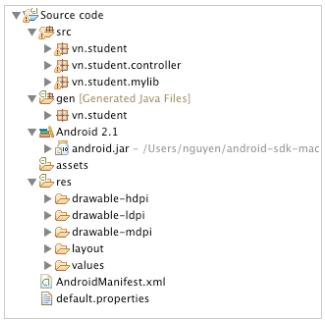
\includegraphics [scale=1] {images/h30.png}
\begin{center}
%\captionsetup{justification=justified, labelsep=period}
\caption{Структура директории и файлов проекта ПО Андроид на Eclipse} \label{img30}
\end{center}
\end{figure}
\textbf{Файл AndroidManifest.xml:}

Этот файл является основой всех Android-приложений, AndroidManifest.xml файл помещается в папке Root и показывает компоненты, которые включены в приложении (activities, services) и как компоненты прикреплены вместе.

При создании файла manifest, необходимо обеспечить свойства пакета, то есть имя пакета Java, используемого в качестве основы для нашего приложения. После ввода имени пакета и, в случае необходимости, в файле manifest, мы можем сократить, например, с классом "com.yourapp.android.search. Someclass", просто пишется: ".Someclass".
\begin{figure}[ht!]
\centering
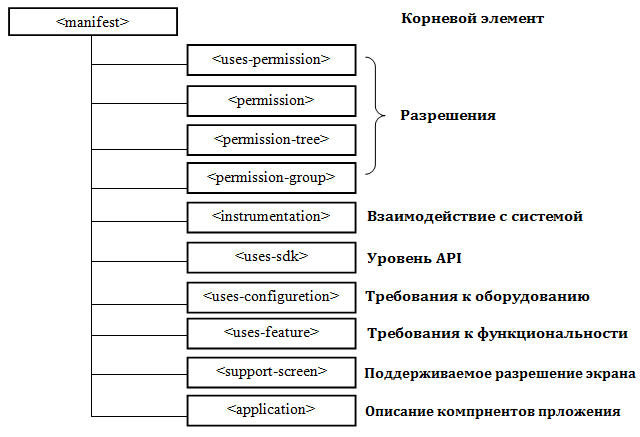
\includegraphics [scale=1] {images/h34.png}
\begin{center}
%\captionsetup{justification=justified, labelsep=period}
\caption{Структура файла Manifest.} \label{img34}
\end{center}
\end{figure}

\subsection{Библиотеки поддержки для разработки приложений}
\textbf{Библиотека обработки изображений для Android – OpenCV}

OpenCV (Open Computer Vision Library) - библиотека компьютерного зрения, которая распространяется в виде открытого исходного кода. Изначально OpenCV была написана для программ на языке C, но теперь работает на других языках, таких как C ++, Java, Android, IOS. А так же время поддерживает много ОС: Windows, Linux, Android, Mac OS, Cube.

В настоящее время в библиотеке OpenCV существует более 2500 алгоритмов, которые включают в себя совокупность всех алгоритмов компьютерного зрения и машинного обучения. Эти алгоритмы могут быть использованы для обнаружения и распознавания лиц, распознавания объектов и классификации человеческих действий в видео, отслеживать перемещение объектов, извлекать 3D модели объектов, нахождения похожих изображений из базы данных изображений, удаления эффекта красных глаз из изображений, снятых с использованием вспышки, отслеживания движения глаз и т.д.

Структура OpenCV включает в себя 4 основных компонента:
\begin{figure}[ht!]
\centering
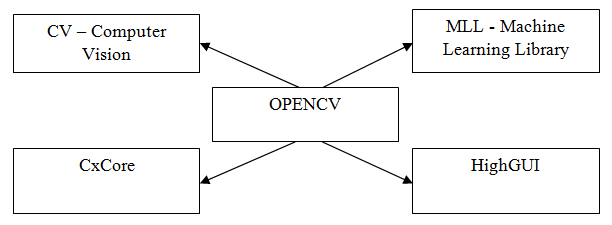
\includegraphics [scale=1] {images/h31.png}
\begin{center}
%\captionsetup{justification=justified, labelsep=period}
\caption{Структура OpenCV} \label{img31}
\end{center}
\end{figure}


\begin{itemize}
	\item \textbf{CxCore}: Содержит основную структуру, такие как точки, линии, блоки, руки, матриц, и связанные с ними манипуляции низкого уровня;
	\item \textbf{MLL} (Machine Learning Library) является библиотекой машинного обучения, эта библиотека включает в себя много классов статистики и инструментов обработки;
	\item \textbf{CV} (Computer Vision – компьютерное зрение): Содержит множество операций, связанных с обработкой изображений низкого уровня, таких как фильтрация изображений, обнаружение контура, преобразование Фурье и прочее;
	\item \textbf{HighGUI}: Работа с файлами изображений и видео, такие как загрузка изображения, отображения изображений, преобразование форматов.
\end{itemize}
\textbf{Open CV имеет следующие основные модули}:

\begin{itemize}
	\item Opencv core: основная функциональность. Включает в себя базовые структуры, вычисления, ввод и вывод для XML и т.д;
	\item Opencv imgproc: обработка изображений;
	\item Opencv highgui: модуль для создания пользовательского интерфейса;
	\item Opencv feature2d: распознавание и описание плоских примитивов (SURF, FASR и др.);
	\item Opencv video:анализ движения и отслеживание объектов;
	\item Opencv objdetect: обнаружение объектов на изображении;
	\item Opencv ml:модели машинного обучения.	
\end{itemize}

\textbf{Библиотека моделирования 3D – MakeHuman}

MakeHuman - программное обеспечение с открытым исходным кодом, является бесплатным, служит для создания 3D модели человека. MakeHuman прост в использовании и имеет интуитивно понятные параметры, в том числе:

\begin{itemize}
	\item Возраст, пол, рост, вес;
	\item Пропорция тела, форма лица;
	\item Глаза, нос, рот, подбородок, уши, шея ...
	\item Руки, ноги

\end{itemize}

Это приложение разработано с использованием 3D-технологий. Создание начинается с формы человека, а затем преобразуется во множество различных персонажей, в том числе мужчин и женщин. Кроме того, мы можем преобразовать 3D модели из формы ребенка в юношу, взрослого и пожилого человека. Начиная с первой версии, MakeHuman использовало уникальные сетки.  

\textbf{Библиотека поддержки моделирования min3D}
\begin{figure}[ht!]
\centering
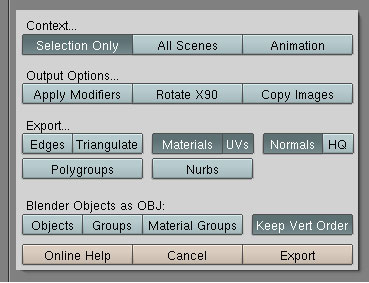
\includegraphics [scale=1] {images/h32.png}
\begin{center}
%\captionsetup{justification=justified, labelsep=period}
\caption{Структура библиотеки моделирования min3D} \label{img32}
\end{center}
\end{figure}

Библиотека Min3D имеет открытый исходный код, разработанный для операционной системы Android для отображения 3D-моделей. Она использует инструмент поддержки OpenGL версий 1.0/1.1. Min3D совместим с OpenGL API, предоставляет удобную и полезную библиотеку для приложений моделирования. Библиотека Min3D легко восстановит 3D-модели объекта. Min3D работает на следующих файлах: Wavefront OBJ, 3DS, MD2.

В данной работе используется сочетание двух библиотек MakeHuman и Min3D для создания шаблонов 3D-моделей человеческого тела. Эти шаблоны описаны в двух файлах с расширениями *.mtl и *.obj. Эти файлы хранятся в папке Андроида (project/res/raw). 


\begin{itemize}
	\item Файлы *.obj содержат данные, описывающие 3D-модели в формате текста, а также другую информацию об объекте. Файлы *.obj просты в использовании и полезны для хранения и отображения 3D-модели любого объекта;
	\item Файлы *.mtl содержат информацию текстур объектов. 
\end{itemize}
Оба файла * .obj и * .mtl являются конечным результатом конструкции 3D-модели человека на основе результата извлечения антропометрических признаков системы компьютерного зрения, предложены библиотека MakeHuman и входные данные для отображения на устройствах Android сгенерированные с помощью библиотеки min3D.




